\section{I²C}

\subsection{Verkablung über Breadboard (Wohlrab)}

Zur ersten Funktionsüberprüfung des Sensors wurde eine einfache Testschaltung auf einem Breadboard aufgebaut. 
Dabei wurde der Raspberry Pi über die GPIO-Pins mit dem Breadboard verbunden. 
Im nächsten Schritt wurden die Anschlüsse des Ultraschallsensors mit den entsprechenden Leitungen auf dem Breadboard verbunden, um eine grundlegende Funktionalität und Signalübertragung sicherzustellen.

\subsection{Einrichten des Raspberry Pi (Wohlrab)}

Um mit den Sensoren über das I²C-Protokoll kommunizieren zu können, muss der Raspberry Pi entsprechend konfiguriert werden. 
Dazu muss zunächst die I²C-Schnittstelle aktiviert werden, was über die Kommandozeile des Raspberry Pi erfolgt. 
Dies kann mithilfe des Konfigurationswerkzeugs „raspi-config“ durchgeführt werden. 
Dort muss unter dem Punkt „Interfacing Options“ die Option „I2C“ aktiviert werden.

\subsection{Testing der I²C Verbindung (Wohlrab)}

Zur Verifizierung der I²C-Kommunikation zwischen Mikrocontroller und Sensor wurde ein einfaches Python-Skript entwickelt. 
Das Skript initialisiert zunächst die I²C-Schnittstelle und überprüft die Erreichbarkeit des Sensors, indem es die I²C-Adressen ausliest.
Anschließend wird ein einfacher Steuerbefehl an den Sensor gesendet und die Antwort des Sensors ausgewertet. 
Durch diese bidirektionale Kommunikation kann sichergestellt werden, dass sowohl das Senden von Befehlen als auch das Empfangen von Daten über die I²C-Verbindung zuverlässig funktioniert.

\subsection{Ansteuerung der Sensoren über die Software (Wohlrab)}

Um mit einem Sensor über die I²C-Schnittstelle zu kommunizieren, muss zunächst dessen spezifische I²C-Adresse bekannt sein. 
Diese ist in der Regel im Datenblatt des Sensors dokumentiert. 
Alternativ kann die Adresse mit dem Kommandozeilen-Tool „i2cdetect” ermittelt werden. 
Dieses listet die am I²C-Bus angeschlossenen Geräte und deren Adressen auf.
Zur Verbesserung der Lesbarkeit und Flexibilität des Quellcodes werden die I²C-Adressen der Sensoren mittels Define-Anweisungen im Code festgelegt. 
Dies ermöglicht eine einfache Anpassung bei Änderungen der Sensoradressen.
Die Kommunikation beginnt mit dem Öffnen des entsprechenden I²C-Kanals und dem Aufbau einer Verbindung zum Sensor über dessen Adresse. 
Der Datenaustausch erfolgt dabei in einem standardisierten Ablauf: 
Zunächst wird das Zielregister des Sensors adressiert und anschließend werden Befehle oder Daten übertragen. 
Nach Abschluss der Kommunikation wird der I²C-Kanal ordnungsgemäß geschlossen, um die Verbindung zu beenden und Ressourcen freizugeben.

\subsection{Finale Verkabelung (Wohlrab)}

Die endgültige Umsetzung der I²C-Bus-Verkabelung erfolgte mithilfe von Dupont-Crimp-Verbindungen. 
Diese gewährleisten eine individuelle und dennoch zuverlässige Verbindung der Komponenten. 
Wie in Abbildung~\ref{fig:i2c_stecker} dargestellt, wurden auf der Seite des Raspberry Pi sämtliche Leitungen in einem gemeinsamen Stecker zusammengeführt.
Eine Besonderheit dieser Umsetzung ergibt sich aus den unterschiedlichen Spannungsanforderungen der verwendeten Sensoren: 
Da der Gyroskop-Sensor und der Ultraschallsensor unterschiedliche Versorgungsspannungen benötigen, wurde der Stecker so ausgelegt, dass zwei separate Plusleitungen integriert sind. 
Dadurch kann die Spannungsversorgung der Sensoren individuell gestaltet werden.
Die restlichen Leitungen, insbesondere die Daten- und Taktleitungen des I²C-Busses (SDA und SCL), wurden zusammengeführt und in den gemeinsamen Anschluss integriert. 
Auf der Seite der Sensoren verzweigt sich der Bus in zwei separate Stecker, die jeweils mit den entsprechenden Sensoren verbunden sind. 
Diese Struktur ermöglicht eine übersichtliche und modulare Verbindung der Sensoren bei gleichzeitiger Wahrung der elektrischen Anforderungen.
\begin{figure}[ht]
    \centering
    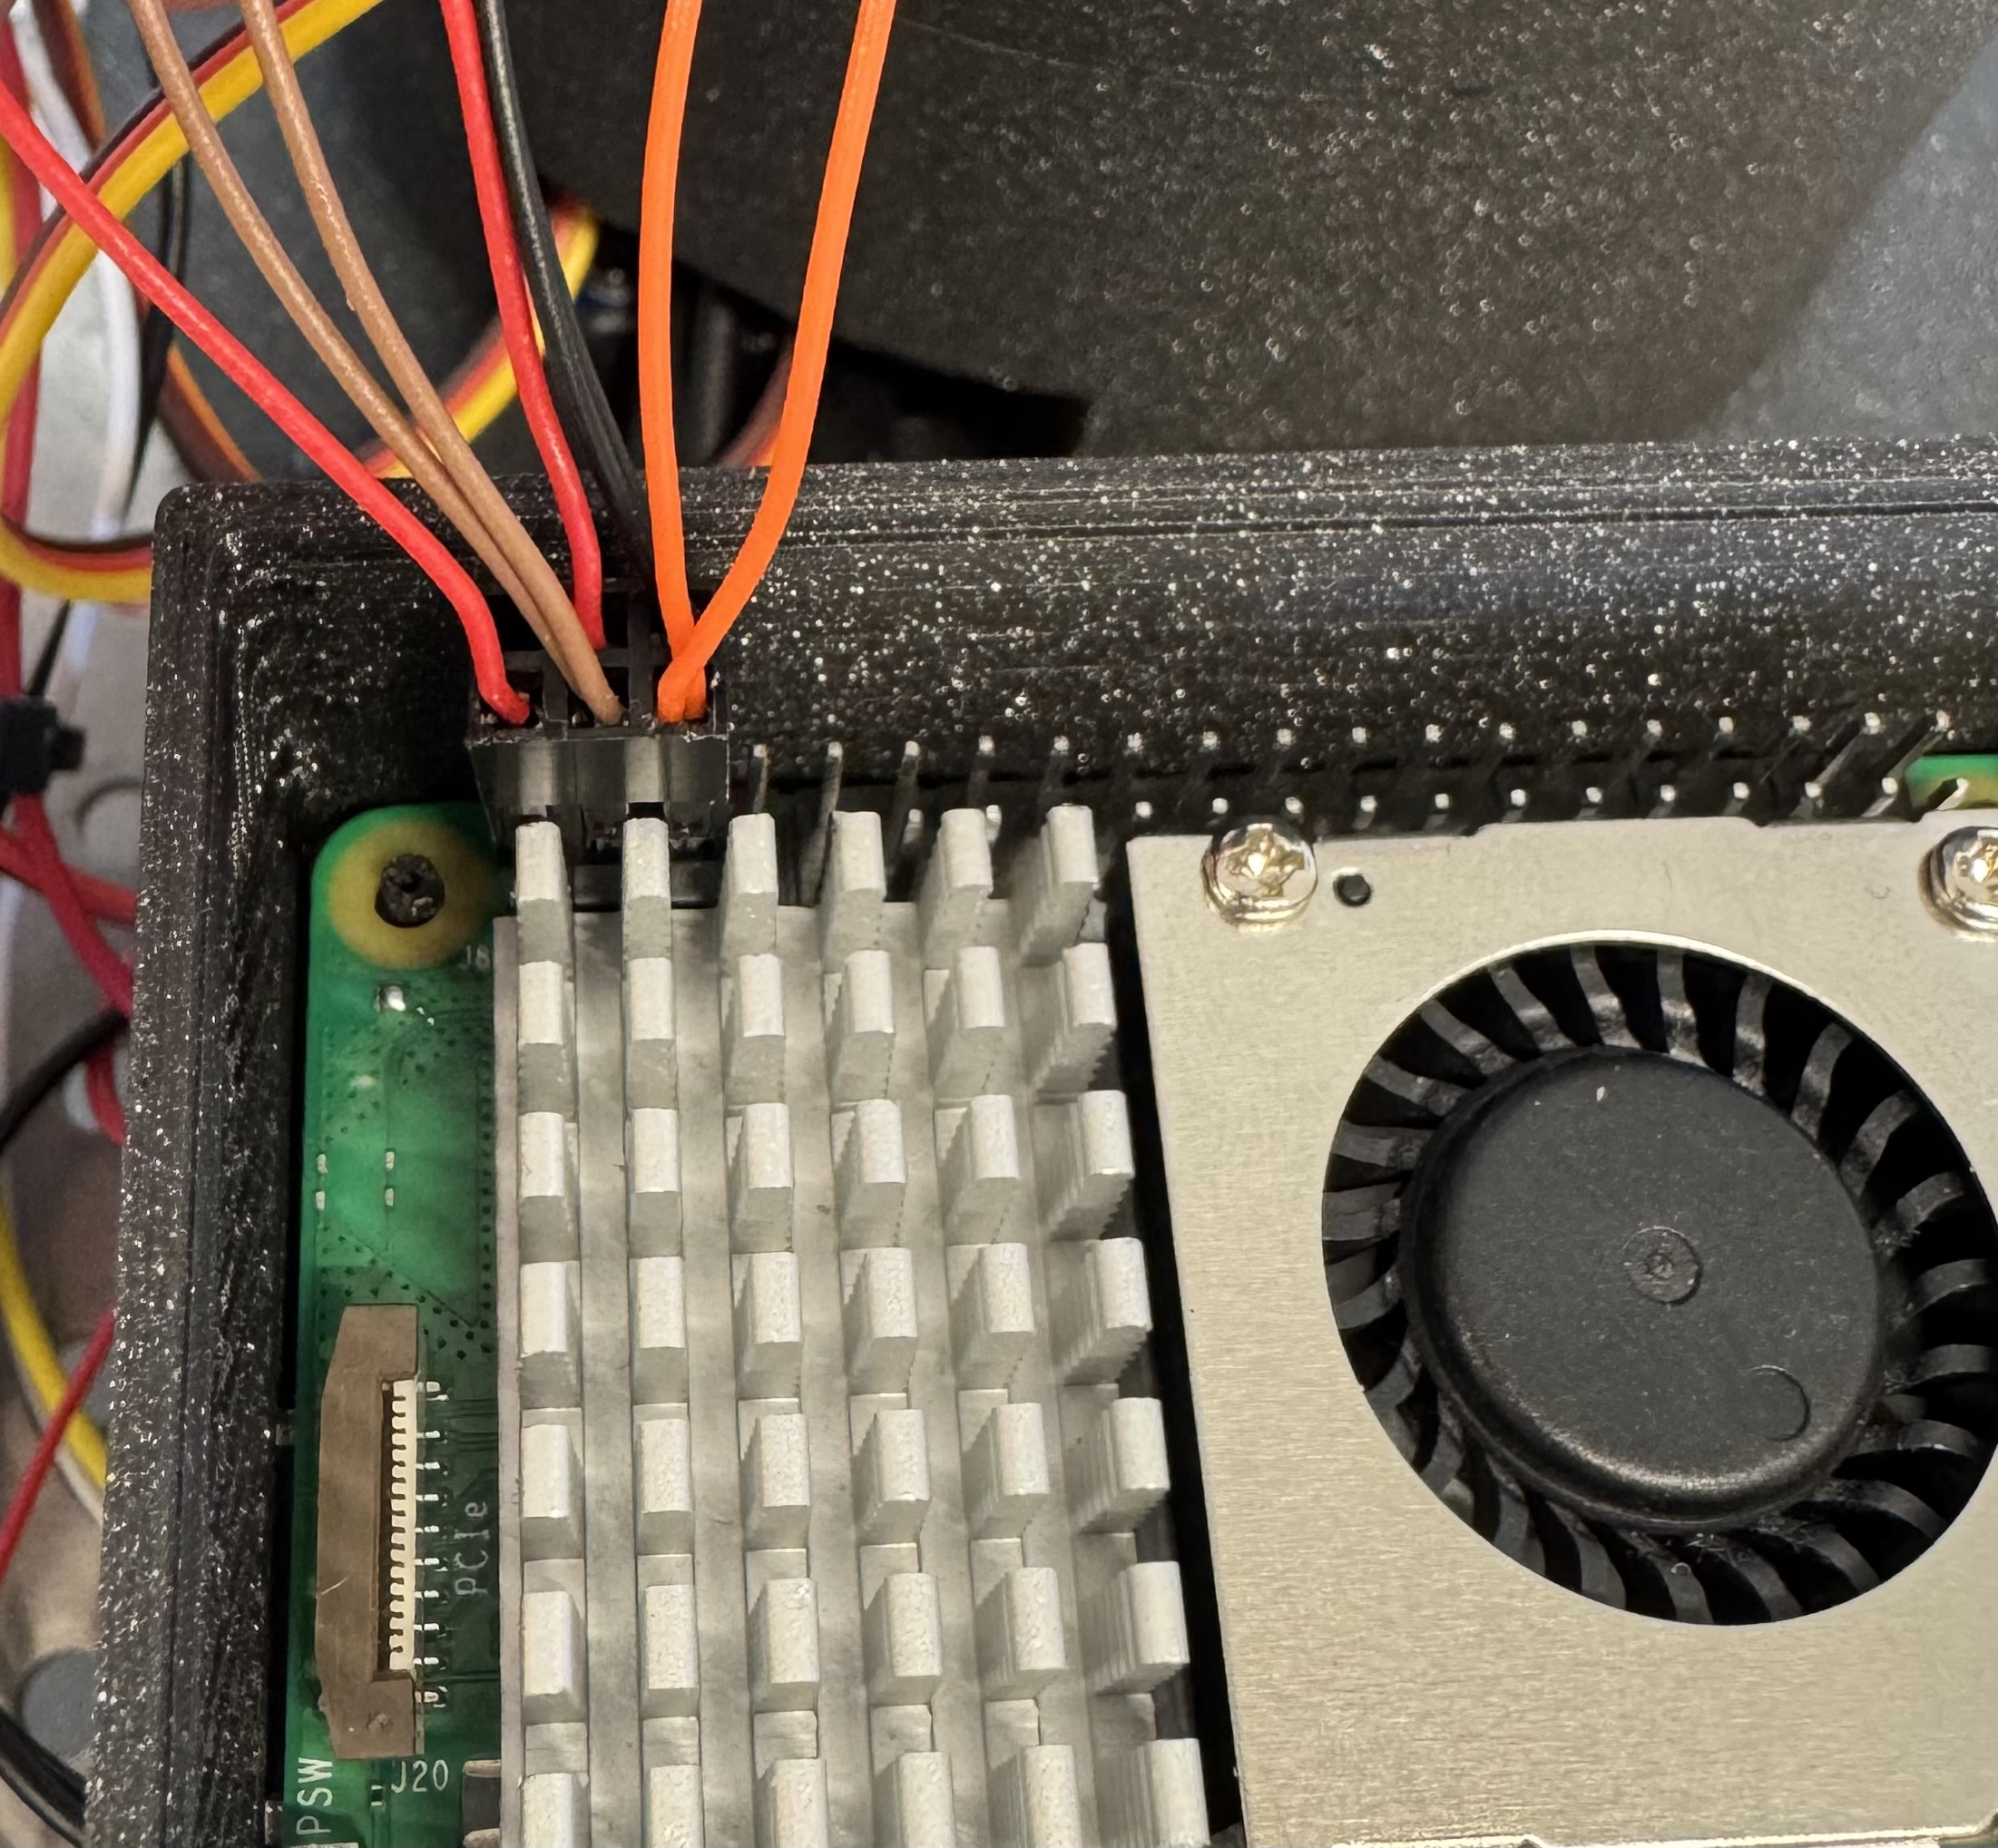
\includegraphics[width=0.5\textwidth, keepaspectratio]{images/wohlrab_i2c_stecker.png}
    \caption{Dupont-Crimp-Stecker der finalen I²C-Verkabelung}
    \label{fig:i2c_stecker}
\end{figure}